\begin{frame}{Implementación}
  \framesubtitle{Motor de simulación}
  \begin{algorithmic}[1]
    \Require $\vv{r}_i(0)$, $\vv{v}_i(0)$, target final y $v_{di}$ de cada peatón, $t_f$, $dt$, $dt_2$
    \State $n \gets \mathrm{round}(dt_2/dt)$, \quad $dt \gets dt_2/n$
    \For{$k = 1,\, 2,\, \dots,\, t_f/dt_2$}
      \For{$n$ pasos de integración}
        \For{cada peatón $i$}
          \State $\vv{e}^{\,target}_i \gets$ hacia target temporal si hay conflicto; si no, hacia target final
          \State $\vv{F}_i \gets \vv{F}_{Di} + \vv{F}_{Gi}$
        \EndFor
        \State $\vv{v}_i \gets \vv{v}_i + (\vv{F}_i/m_i)\,dt$
        \State $\vv{r}_i \gets \vv{r}_i + \vv{v}_i\,dt$
      \EndFor
      \State guardar $t = k\,dt_2$, $\vv{r}_i$, $\vv{v}_i$
    \EndFor
  \end{algorithmic}
\end{frame}

\begin{frame}{Implementación}
  \framesubtitle{Elección del paso de simulación}
  \centering
  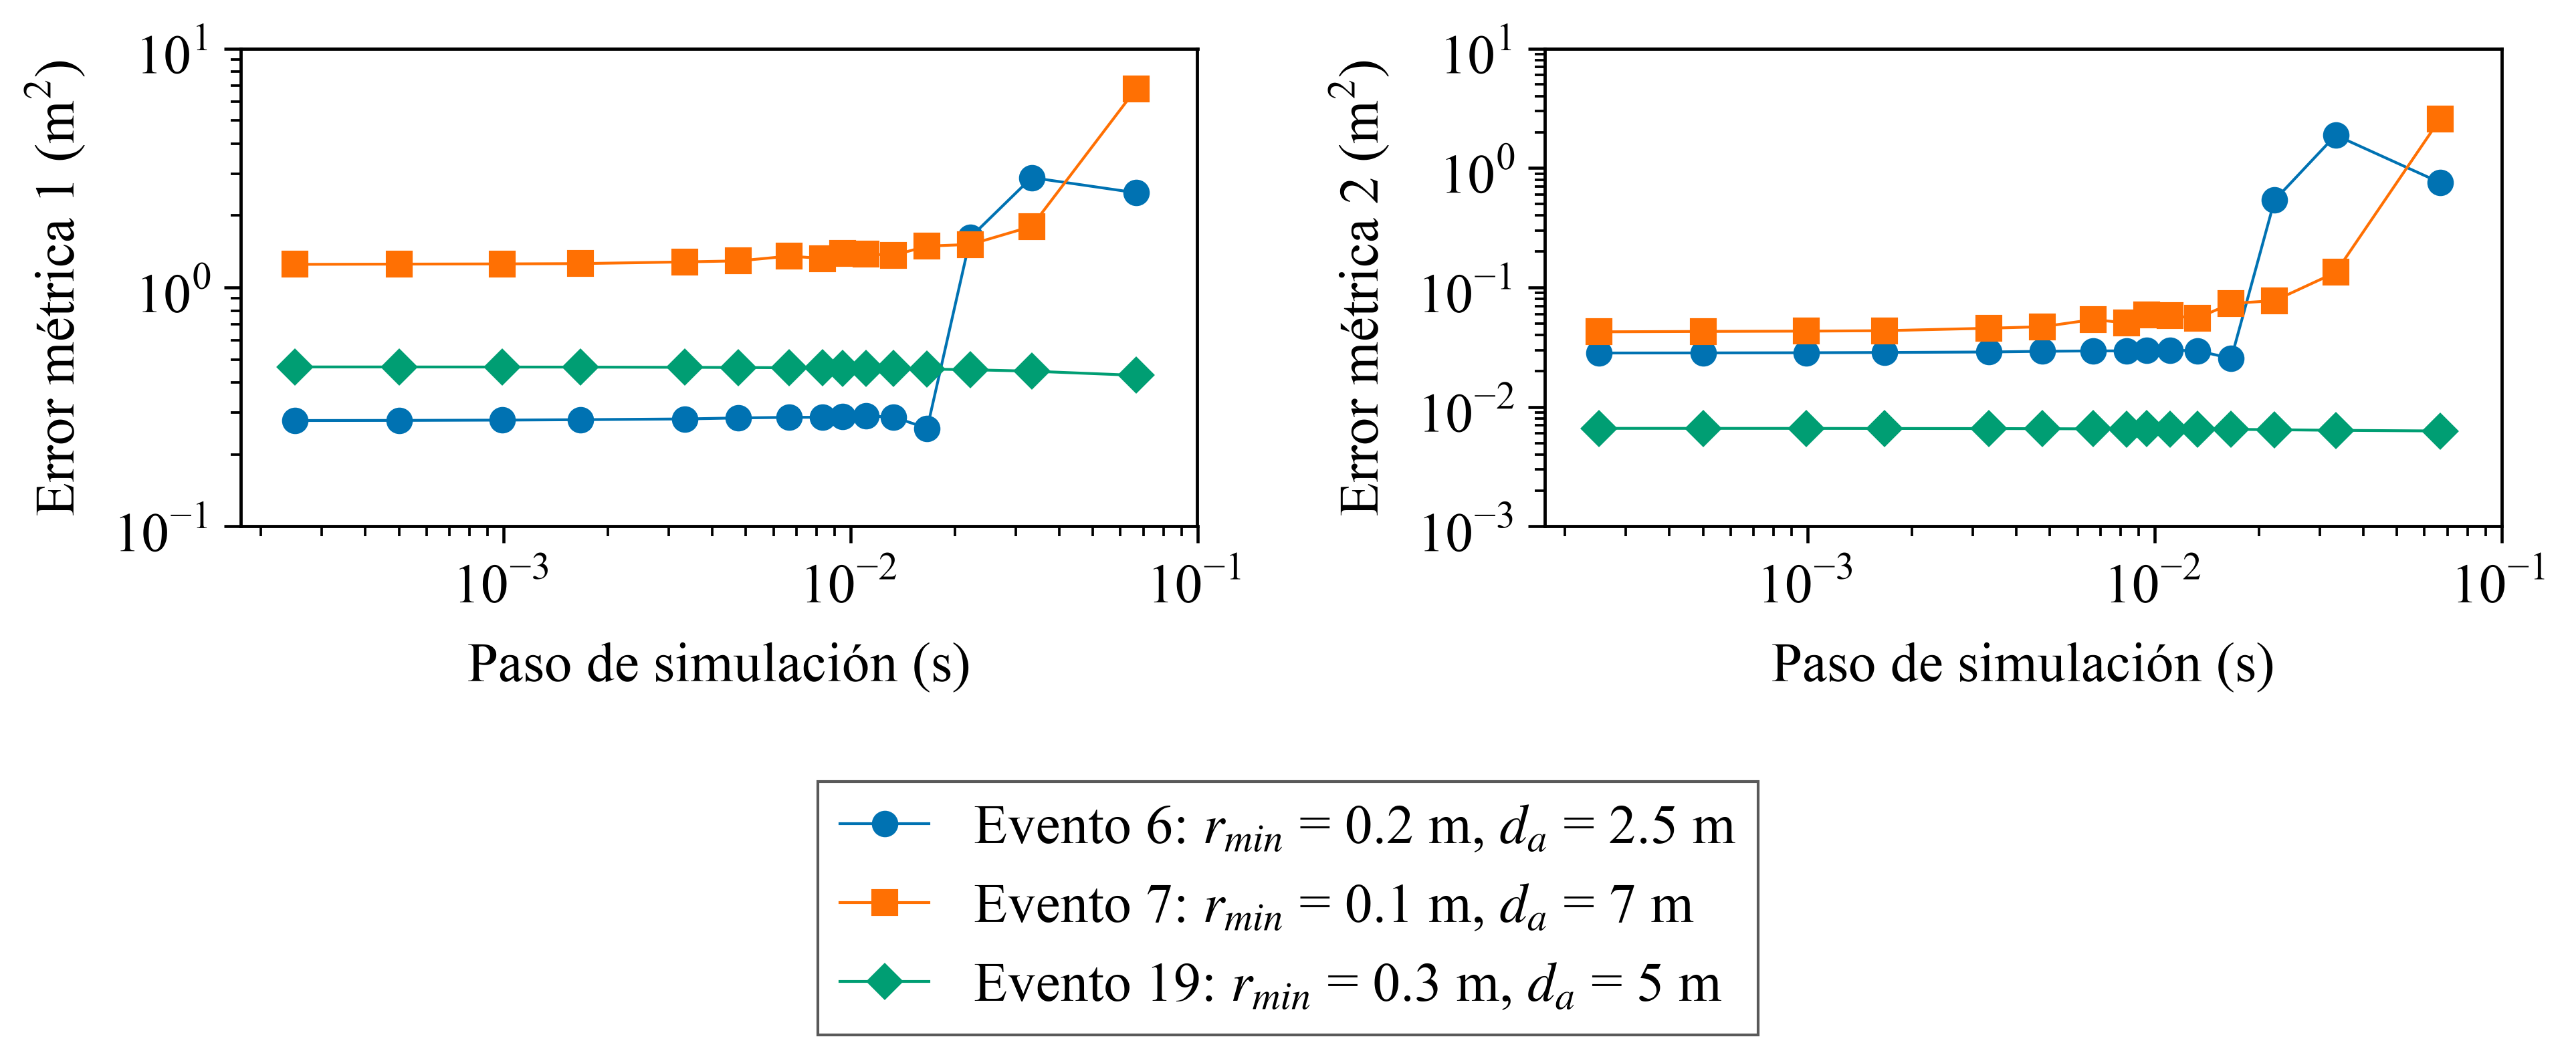
\includegraphics[width=\linewidth,height=0.70\textheight,keepaspectratio]{dt_convergencia.png}

  \vspace{4pt}
  {\large Paso de simulación $dt = 10^{-3}\uni{s}$; \quad paso para guardar estado $dt_2 = \Delta t_{exp}$}
\end{frame}
